\documentclass[nobib]{tufte-handout}

\usepackage{amsmath}
%\setlength{\thinmuskip}{6mu minus 2mu} %3mu
%\setlength{\medmuskip}{8mu plus 4mu minus 8mu} %4mu plus 2mu minus 4mu
%\setlength{\thickmuskip}{10mu plus 10mu minus 5mu} %5mu plus 5mu
%\thinmuskip = 4mu minus 2mu
%\medmuskip = 6mu plus 4mu minus 8mu
%\thickmuskip = 8mu plus 10mu minus 5mu

\usepackage{microtype}
\usepackage{booktabs}
\usepackage{units}
\usepackage{hyperref}
\usepackage{natbib}



% Set up the images/graphics package
\usepackage{graphicx}
\setkeys{Gin}{width=\linewidth,totalheight=\textheight,keepaspectratio}
\graphicspath{{graphics/}}

\title{{Term paper for Acoustic Phonetics WS20/21\\\cite{wang2015supervised} Summary and Terminology}}


\author{Jingwen LI and Kuan TANG
\thanks{
Seminar f\"ur Sprachwissenschaft, Eberhard Karls Universit\"at T\"ubingen \\
{\it{jingwen.li/kuan.tang@student.uni-tuebingen.de}}}}
\date{28. Mar 2021}

% \usepackage{fancyvrb}
% \fvset{fontsize=\normalsize}

% Small sections of multiple columns
\usepackage{multicol}

% Provides paragraphs of dummy text
\usepackage{lipsum}

% % These commands are used to pretty-print LaTeX commands
% \newcommand{\doccmd}[1]{\texttt{\textbackslash#1}}% command name -- adds backslash automatically
% \newcommand{\docopt}[1]{\ensuremath{\langle}\textrm{\textit{#1}}\ensuremath{\rangle}}% optional command argument
% \newcommand{\docarg}[1]{\textrm{\textit{#1}}}% (required) command argument
% \newenvironment{docspec}{\begin{quote}\noindent}{\end{quote}}% command specification environment
% \newcommand{\docenv}[1]{\textsf{#1}}% environment name
% \newcommand{\docpkg}[1]{\texttt{#1}}% package name
% \newcommand{\doccls}[1]{\texttt{#1}}% document class name
% \newcommand{\docclsopt}[1]{\texttt{#1}}% document class option name

\begin{document}
\maketitle

\begin{abstract}
\noindent This term paper aims to introduce the main concepts and methods of \cite{wang2015supervised}. The content and authorship of this paper as follows: In the first section, Kuan summaries the whole paper in general, and make clear that the research questions, methodology, and experimental results in \cite{wang2015supervised}. In section 2, Jingwen introduces the theoretical frameworks for both Supervised EP detection and Unsupervised EP discovery respectively as well as simple and vivid examples to explain the core model structures used in this paper. On this basis, Kuan gives more details about the concepts of clustering and metrics and the applications of both in the paper in section 3, and then put forward two questions after reading the full text in the end.
\end{abstract}


\bigskip
\section{1. \textbf{Summary}}

How to apply the Speech Processing Technology in Second Language Learning (SLL)? How to generate informative feedback for Second Language Learners (SLLs) to improve their pronunciation based on Computer-assisted language learning (CALL)  and Computer-aided pronunciation training (CAPT)\sidenote{Computer-aided pronunciation training (CAPT) aims to analyze the produced utterance to offer feedback to the language learner in the form of quantitative or qualitative evaluations of the pronunciation proficiency. }? How to offer SLLs not only quantitative measures of language proficiency, but also specific types of errors the they have made? These are three trends which have led to substantial efforts toward CALL to meet the strong demand of SLL. At least two different but closely related Pronunciation error patterns (EPs)\sidenote{Pronunciation error patterns (EPs) are patterns of mispronunciation frequently produced by language learners, and are usually different for different pairs of target and native languages. } tasks in CAPT: First, to derive the EP dictionary for a given L1-L2 pair, or a given L2 but non-specific L1; Second, to verify whether a voice segment produced by a learner is correct, or if it belongs to a specific EP based on the EP dictionary. 



\cite{wang2015supervised} propose two new novel frameworks for both Supervised Error Patterns Detection and Unsupervised EP Discovery.  For supervised EP detection,  they use hierarchical multi-layer perceptrons (MLPs) as the EP classifiers to be integrated with the baseline using HMM/GMM in a two-pass Viterbi decoding architecture.  As for unsupervised EP discovery, they  use the Hierarchical Agglomerative Clustering (HAC) algorithm to explore sub-segmental variation within phoneme segments and produce fixed-length segment-level feature vectors to distinguish different EPs. 

They tested K-means \sidenote{Assuming a known number of EPs} and the Gaussian mixture model with the minimum description length principle \sidenote{Estimating an unknown number of EPs} for EP discovery.  And they also propose to use the universal phoneme posteriorgram (UPP), derived from an MLP trained on corpora of mixed languages, as frame-level features in both supervised detection and unsupervised discovery of EPs. 

Preliminary experiments offered very encouraging results.  As the experimental results shown, comparing with other models, the new framework enhances the power of EP diagnosis, and using UPP achieves the best performance and is useful in analyzing the mispronunciation produced by language learners.





\bigskip
\section{2. \textbf{Theoretical Framework}}
\subsection{2.1 \textbf{Error Patterns}}

\textbf{Error patterns} (EPs) in pronunciation training are frequently encountered mispronunciations that have intrinsic commonalities. In other words, mispronunciations of the same error pattern usually display a high level of intra-group similarity, although they can still be very close to the canonical pronunciation or other EPs.\\

EPs can help give more informative and targeted feedbacks in pronunciation training. For example, language learners of different L1s may all pronounce the word wrong (wrong as in deviation from the canonical pronunciation), but their mispronunciations can be incorrect in different ways. It would be more helpful if the CAPT system can provide feedbacks that are specific enough to show the area of improvement. EPs answer the question \textbf{\textit{"In what way is the given pronunciation wrong?"}} instead of simply stating it as an incorrect pronunciation.\\


\subsection{2.1.1 \textbf{Supervised EP Detection and Unsupervised EP Discovery}}
\textbf{Supervised EP detection}, the most commonly used technique, relies on linguistic expertise of not only the target language, but also the L1s of the learners. Thus defining a full-coverage EP dictionary for different language pairs or mixed languages can be very expensive. As explained above, EPs are similar to their canonical pronunciations. Apart from that, EPs that deviates from the same standard native pronunciation are also similar to each other, making EP detection a rather difficult task even if EP dictionaries can be provided, either generated manually or automatically derived (the task of \textbf{unsupervised EP discovery}). Unsupervised EP discovery aims to derive EPs from corpora directly, without language-based knowledge as precursor. \\

To put it simply, supervised EP detection is like putting pronunciation instances into a divided space, like the box displayed in Figure \ref{fig:box}, each cell is an EP advised by experts. The division of the space depends on the training of the model. On the other hand, unsupervised EP discovery do not presuppose the boundaries or the number of EPs\sidenote{except K-means} (at first). Take \textbf{Hierarchical Agglomerative Clustering} (HAC) as an example, the HAC algorithm starts with each instance in its own cluster and then simply compares the instances using distance\sidenote{There are many distance measures to choose from, to name a few, Euclidean distance, Manhattan distance...} between them in high-dimensional space, the most similar instances are grouped together, until all instances are in the same group. Categories/clusters are in this sense "self-organised" in a bottom-up manner and can be adjusted depending on the desired granularity. This is where human make decisions, a high cut-off at the resulting dendrogram in Figure \ref{fig:dendro} means fewer classes while a low cut-off produces more classes. 
\bigskip
\begin{marginfigure}
  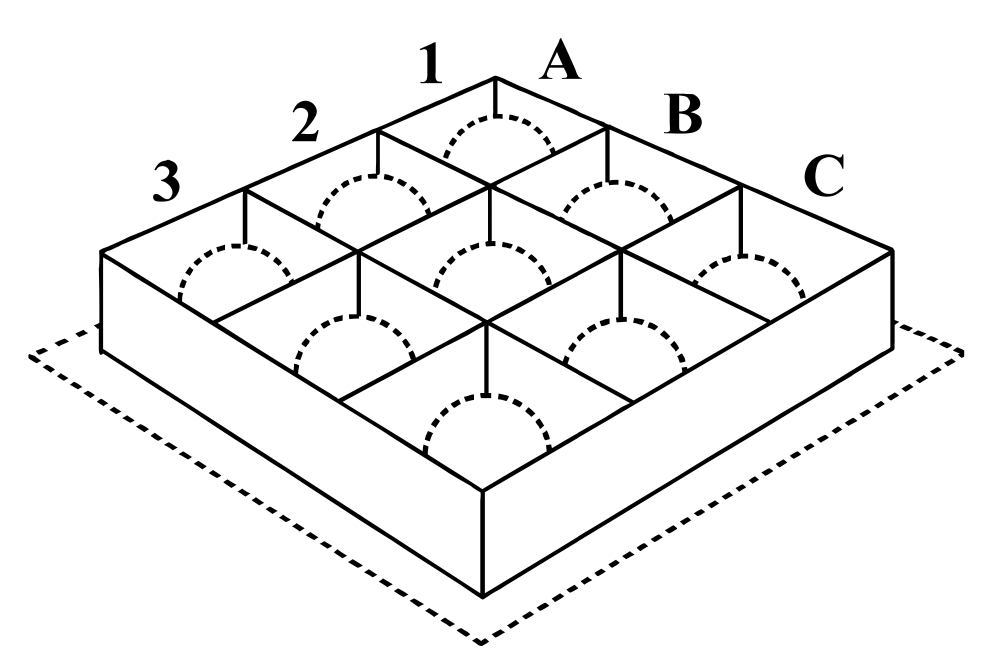
\includegraphics{box.png}
  \caption{A divided box, adopted from p.9 of \url{http://fanfoyan.com/audio/naga.pdf}}
  \label{fig:box}
\end{marginfigure}
\vspace{5em}
\begin{figure}
  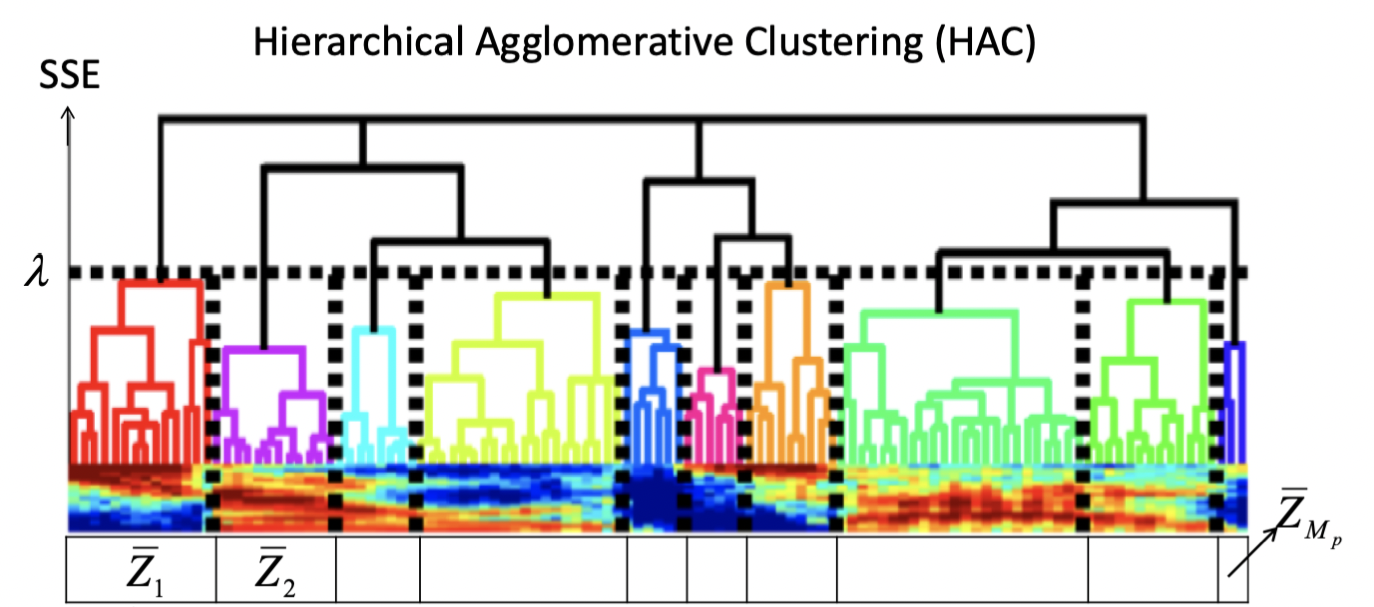
\includegraphics{dendro.png}
  \caption{Dendrogram resulting from HAC, adopted from \cite{wang2015supervised}}
  \label{fig:dendro}
\end{figure}

\subsection{2.2 \textbf{Heterogeneous Initialization of Acoustic Modeling of EPs}}

In supervised detection of EPs, an \textbf{acoustic model} (AM) is needed for each EP. \cite{wang2015supervised} asked language teachers to create an extensive set of 152 EPs, whose descriptions are based on phonemes of Chinese and English. For example, \textit{l\_000} represents the canonical pronunciation of l, while \textit{l\_010} is defined as something pronounced like the English \textit{l}. Since EPs are defined using a  \textbf{\textit{"pronounced-as"}} relationship\sidenote{Notice that the \textbf{\textit{"pronounced-as"}} relationship only describes a pronunciation instance and has nothing to do with the learners' L1.}, it became natural to use existing acoustic models for phonemes as a starting point. Duplicates of phoneme models trained for other corpora are used as the initial EP models, this process is referred to as \textbf{\textit{heterogeneous model initialization}}. A comparison of \textit{heterogeneous model initialization} and \textbf{\textit{homogeneous model initialization}} is illustrated in Figure \ref{fig:init}, where a clear benefit of heterogenous initialization can be seen: Without any anchor points, apart from the experience and knowledge of language teachers, different EPs of the same canonical pronunciation are hard to locate with respect to the correct pronunciation (homogeneous) in the conceptual pronunciation space, let alone to describe them in a human-understandable way, which also makes it almost impossible for human annotators to create target labels. Heterogenous initialization provides the ground to describe the error patterns, which facilitates human understanding as well as acoustic modeling.

\begin{figure}
  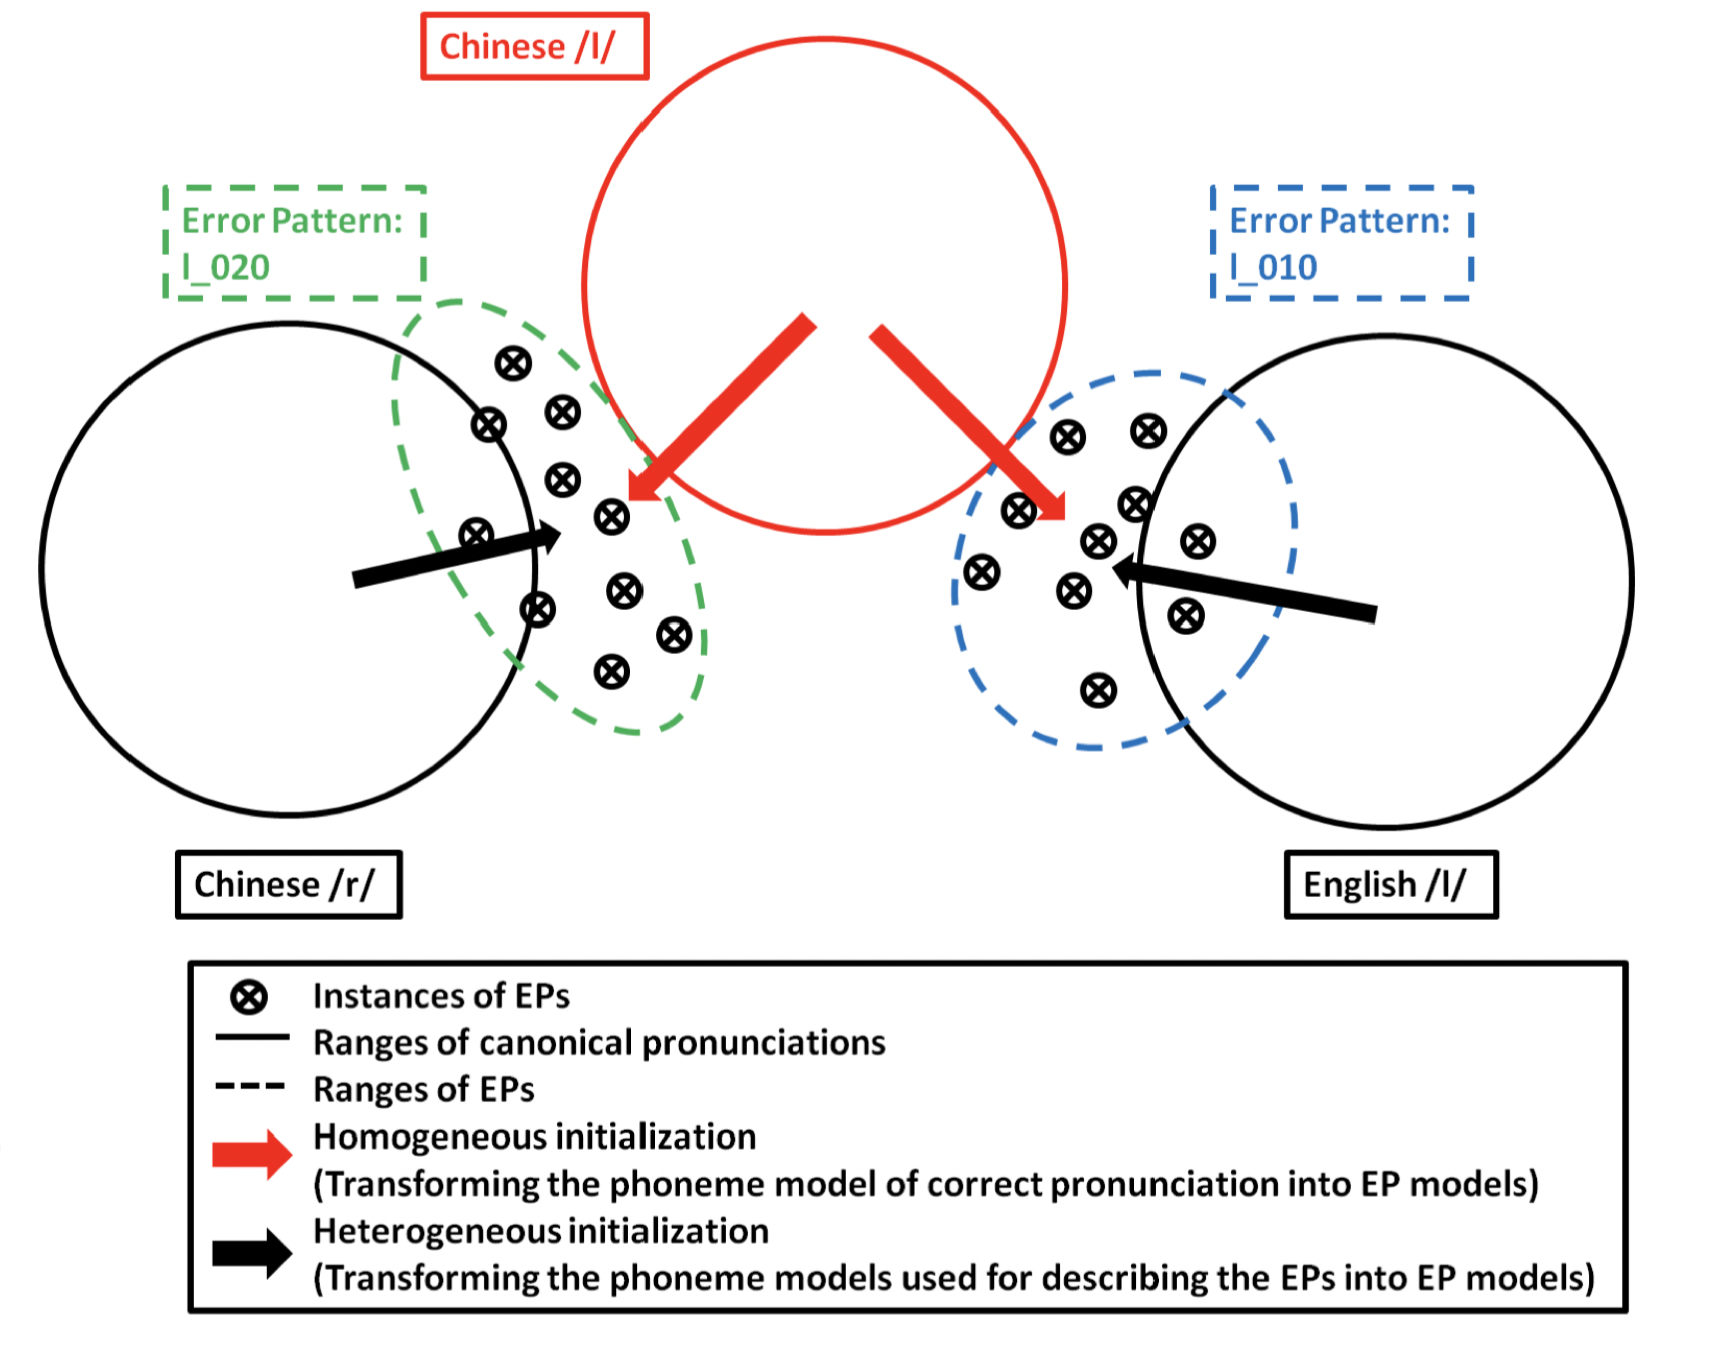
\includegraphics{init.png}
  \caption{Homogeneous and heterogeneous initialization for acoustic modeling
of EPs in the conceptual pronunciation space, adopted from \cite{wang2015supervised}}
  \label{fig:init}
\end{figure}

\subsection{2.3 \textbf{From Perceptrons to Multilayer Perceptrons}}

A \textbf{Perceptron} is a single-neuron model that acts as a \textbf{binary linear classifier}. It is inspired by the biological neuron and can be seen as an abstraction of it. The perceptron receives a real-valued feature vector as input, it also has a weight vector associated with the input vector, which is to be trained. A weighted sum is calculated and passed into an activation function before the output layer. There are varies kinds of activation functions, they help normalise the weighted sum to a range between 0 and 1, or, in some cases, -1 and 1. Like the biological neuron needs an action potential above the threshold of -55 mA to "fire", the perceptron neuron uses the activation function and decides whether to pass on the output or not (acting like a gate), or, in the case of a binary classifier, it decides if the input belongs to a class or not. In the case of the example below, a step function is used where 0 is the threshold, everything above 0 is mapped to 1 and 0 otherwise. \\
\begin{figure*}[h!]
  \centering
  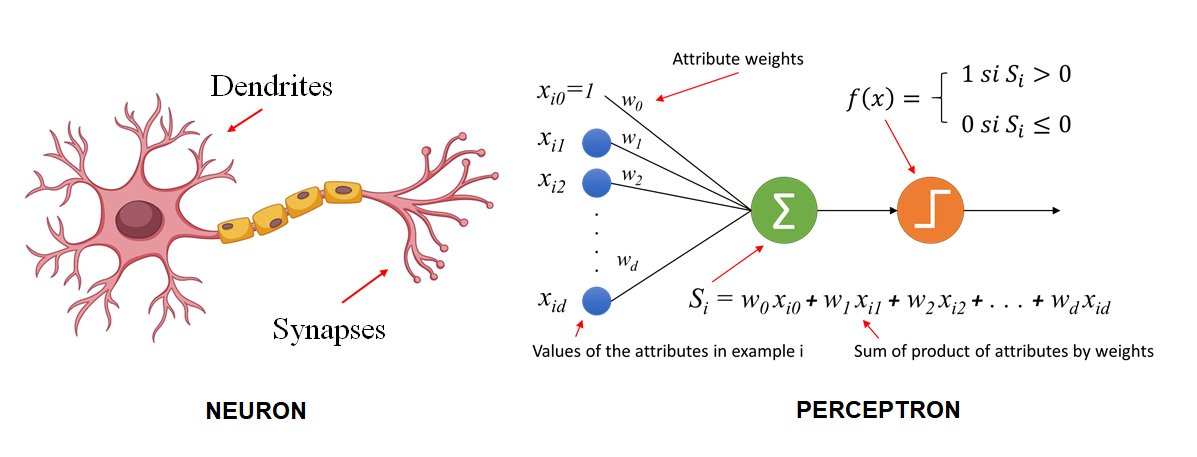
\includegraphics{perceptron1.png}
  \caption{biological neuron vs. perceptron, adopted from \cite{IF:perceptron}}
\end{figure*}
As suggested by the name, \textbf{multilayer perceptrons} (MLPs) have more than one (usually fully connected) layers. The most simple schematic MLP structure illustrated in Figure \ref{fig:mlp} has one input layer, a hidden layer and an output layer. There can be more than one hidden layers, but usually one is enough. MLPs are a class of feedforward artificial neural network (ANN), with "\textbf{feedforward}" meaning single-way, acyclic movement, just like biological neurons.\\ 
\begin{figure}[h!]
\centering
  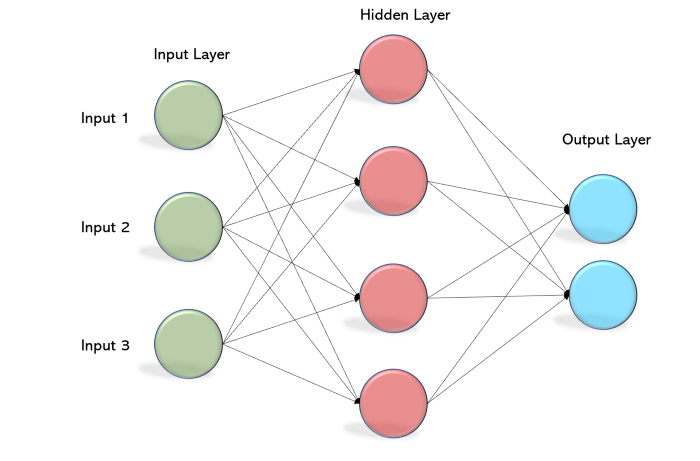
\includegraphics[width=0.9\textwidth]{mlp3.png}
  \caption{A schematic multilayer perceptron model, adopted from \cite{becominghuman:MLP}}
  \label{fig:mlp}
\end{figure}
\newpage
MLPs use \textbf{backpropagation} (BP) as training method, which compares the results to the desired value and adjust the weights that contributed to the error most in each layer using the chain rule. The adjusted weights are used in the next training cycle. The training process terminates when the loss function is minimised.


\subsection{2.4 \textbf{Universal Phoneme Posteriorgram}}
\noindent \textbf{Universal Phoneme Posteriorgram} (UPP) is used as the fundamental frame-level feature of supervised EP discovery in \cite{wang2015supervised}. The motivation behind this has to do with the nature of EPs in language learning. Usually EPs are caused by articulator mechanisms or acoustic phenomena present in the target language but missing from learners' native languages as suggested by \cite{wang2015supervised}. However, the discrepancies between mispronounced instances and canonical pronunciations can be small but still obvious to the native ear. Therefore if one simply compare the pronunciations from learners of mixed languages in the same acoustic space, for example the acoustic space spanned by MFCCs, the pronunciations are usually too close to be distinguished by clustering algorithms. What UPP extraction does is to use an MLP as a posterior probability estimator to span the pronunciation instances by phoneme posteriors. Each frame of MFCC feature is transformed into a vector of posterior probabilities of all predefined phonemes in the training corpora of mixed languages.
\begin{figure}[h!]
\centering
  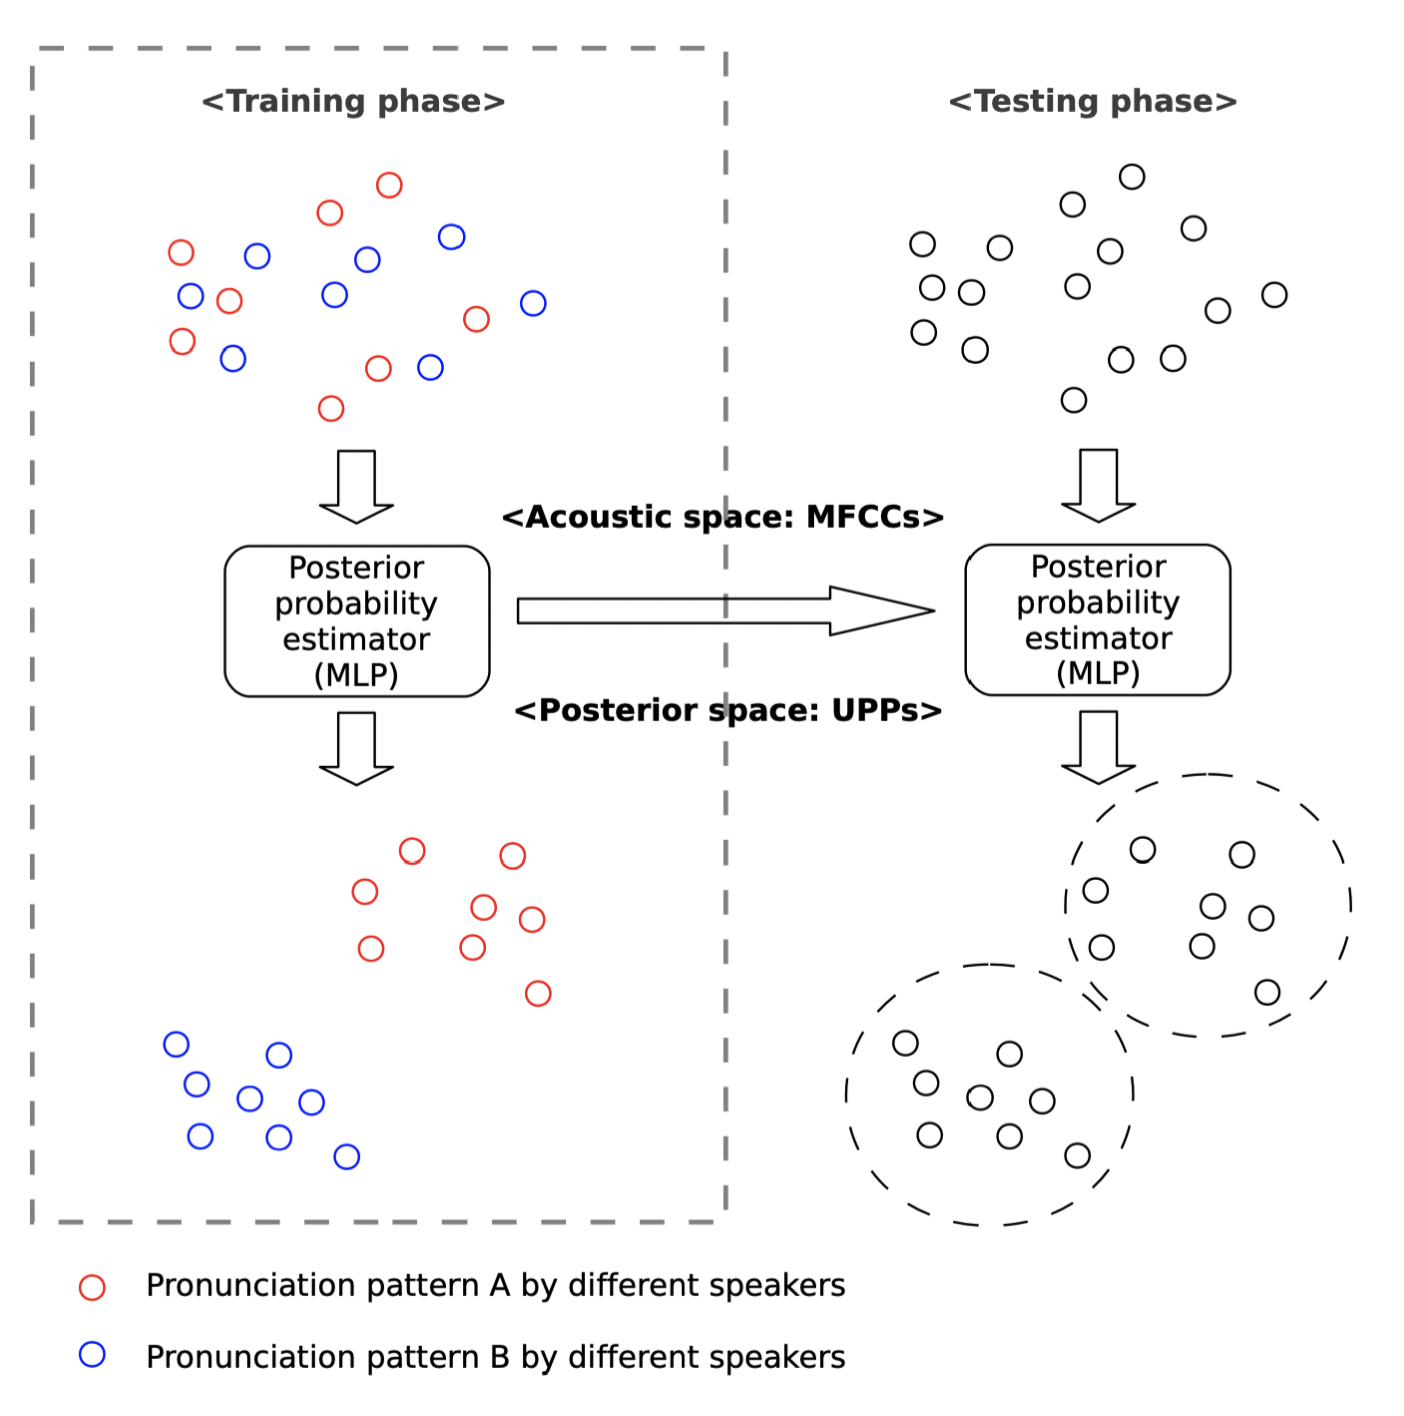
\includegraphics[width=0.81\textwidth]{upp.png}
  \caption{The concept of \textbf{UPP extraction}: mapping from acoustic space (represented by MFCCs) to posterior space (represented by UPPs) using a posterior probability estimator (MLP) so as to better distinguish the pronunciation patterns, adopted from \cite{wang2015supervised}}
  \label{fig:upp}
\end{figure}



\subsection{2.5 \textbf{Hidden Markov Model and Viterbi Decoding}}

\subsection{2.5.1 \textbf{Markov Chains and HMM}}

\begin{marginfigure}
 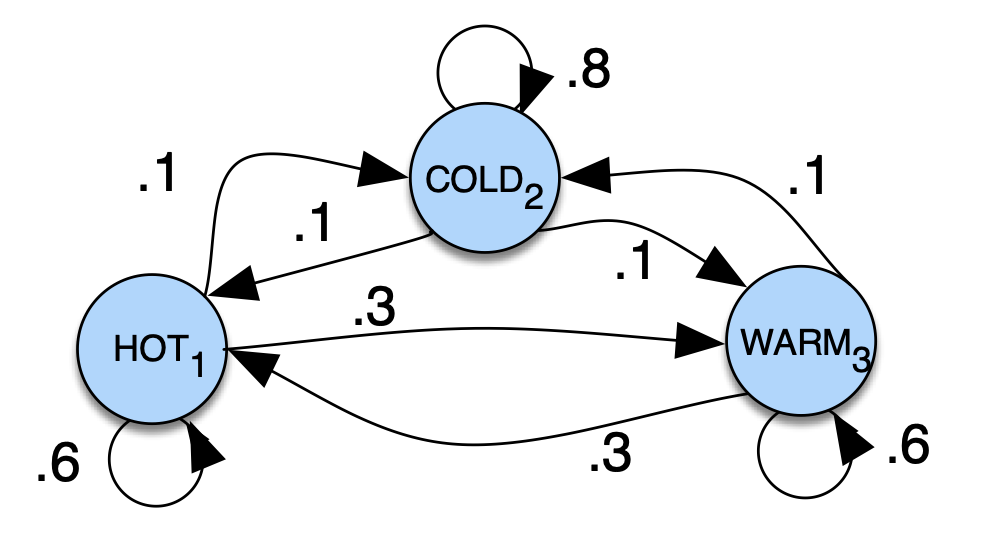
\includegraphics[width=1\textwidth]{chain.png}
  \caption{A Markov chain for weather, showing states and transitions, adopted from \cite{slp}}
  \label{fig:chain}
\end{marginfigure}

\textbf{Markov chains} model the \textbf{probabilities of sequences} of random variables, which are usually termed \textit{states}. The power of the Markov chain lies in the Markov assumption that when predicting the next state, only the current state matters\sidenote{When predicting the future, the past doesn't matter, only the present does.}. Figure \ref{fig:chain} shows a simple Markov chain that models the weather. Each circle represents a state, the arrows represent state transition, with the digits being the transition probability. Let's say today is cold, then we focus on the \textsc{cold} state, there are 3 arrows pointing out from this state, so tomorrow (next state) is either \textsc{cold} again with probability of 0.8, \textsc{hot} or \textsc{warm}, each with probability of 0.1. The probabilities of all possible transitions sum to 1.\\

Hidden Markov Models (HMMs) are Markov chains with \textbf{\textit{hidden states}}. Markov chain is useful when we need to compute the probability for a sequence of observable events, but when what we are interested in cannot be observed directly and we know that it is related with what can be observed, then we use HMM. For example, Jason, as a normal boy, enjoys ice-cream. Although he has ice-cream every day, the amount of ice-creams he has each day differs. Since he is normal, he is more likely to have more ice-creams on hot days and less on cold days. Figure \ref{fig:hmm} shows an HMM that models Jason's ice-cream eating behaviour and the weather. The octagon shows the distribution of the hidden states\sidenote{This distribution can be translated as follows: On any day, the probability that it is a hot day is 0.8, the probability that it is a cold day is 0.2.}. The squares are the \textbf{\textit{emission probabilities}} or \textbf{\textit{observation likelihoods}}\sidenote{Square B${_1}$ can be translated as: On a hot day, it is 20\% chance that Jason eats one ice-cream, 40\% that he eats 2 and 40\% that he eats 3.}. The rest is the same as the Markov chain explained above.\\
\vspace{5em}
\begin{figure}
 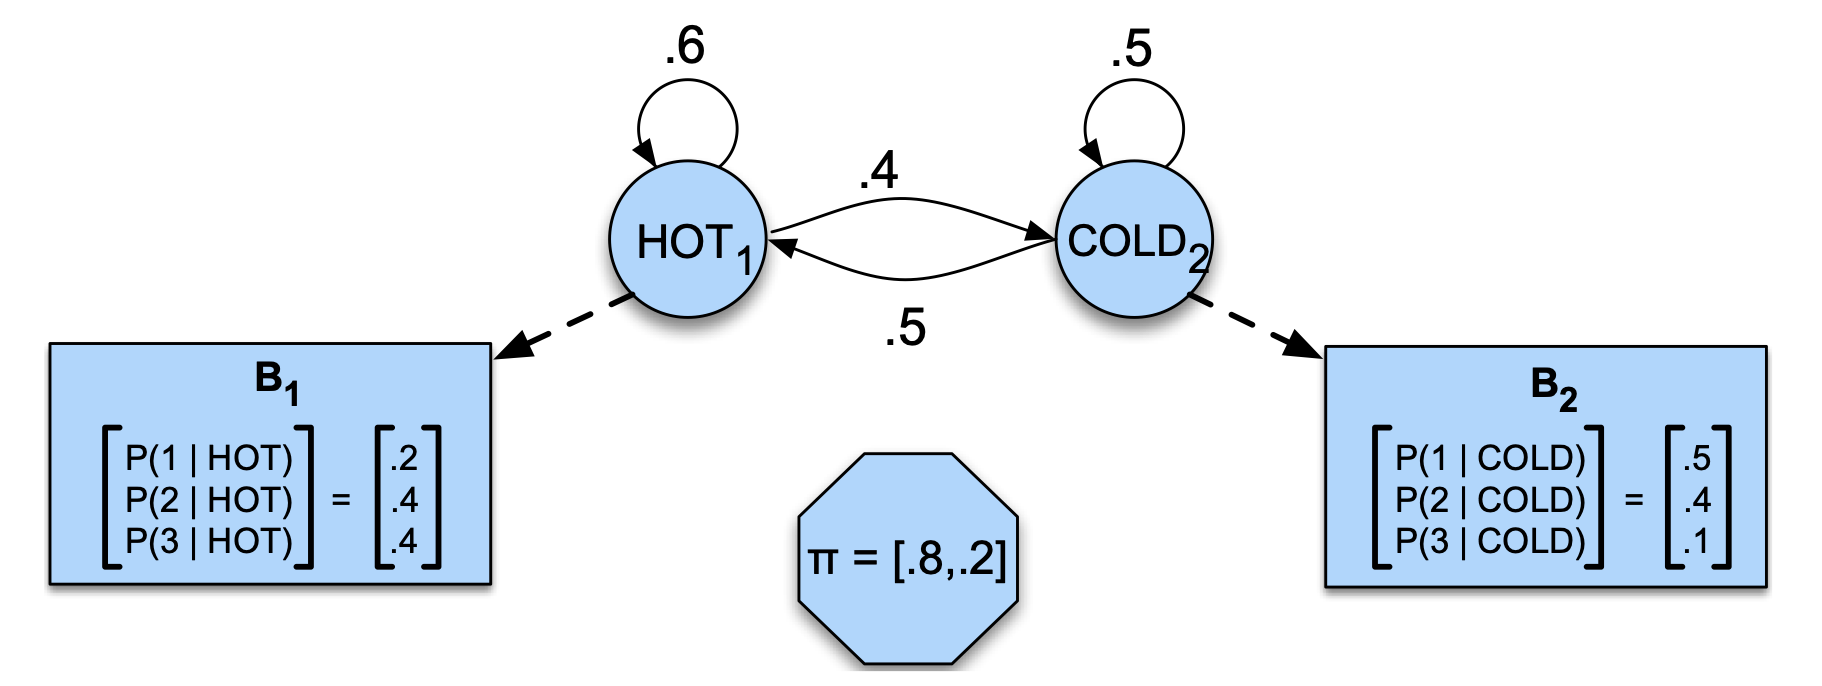
\includegraphics[width=1\textwidth]{hmm.png}
  \caption{A simplistic HMM for relating numbers of ice-creams consumed by Jason each day (observations) to the weather (\textit{Hot(H)} or \textit{Cold(C)}, hidden states), adopted from \cite{slp}}
  \label{fig:hmm}
\end{figure}
Hidden Markov Model (HMM) in Speech Recognition is used to model unit of speech, like words or phones.

\subsection{2.5.1 \textbf{Viterbi Decoding}}

One of the problems that HMM can solve is the \textbf{decoding problem}:\\
\bigskip
\textbf{\textit{Given an observation sequence and an HMM, find the best hidden state sequence.}}\\
\bigskip
Using the ice-cream example above, it means that if for the last 3 days the number of ice-creams Jason had is the observed sequence 3 1 3, what are the weather of these three days most likely like?\\
\textbf{Viterbi algorithm} solves this decoding problem by finding (and remembering) the best (most likely) path at each step. Figure \ref{fig:vi} shows the observations in squares and hidden states in circles. All possible states are drawn, but only the current most likely state is chosen to form the optimal path. For instance, since the initial weather distribution for (\textsc{hot}, \textsc{cold}) is (0.8, 0.2), and on the first day Jason had 3 ice-creams, the probability of the hidden state being \textsc{hot} is the product of 0.8 and the observation likelihood\sidenote{the probability of Jason eating 3 ice-creams given it is a hot day}. Similarly we can calculate the probability of the hidden state being \textsc{cold}. Since \textsc{hot} is 0.32 and \textsc{cold} is 0.02, we pick \textsc{hot}. For the next steps, we don't need the initial weather distribution $\pi$ anymore, we should only consider the current hidden state and the transitions to the next possible hidden states. Using Viterbi decoding, we obtain the thick arrows as the optimal path.

\begin{figure*}
 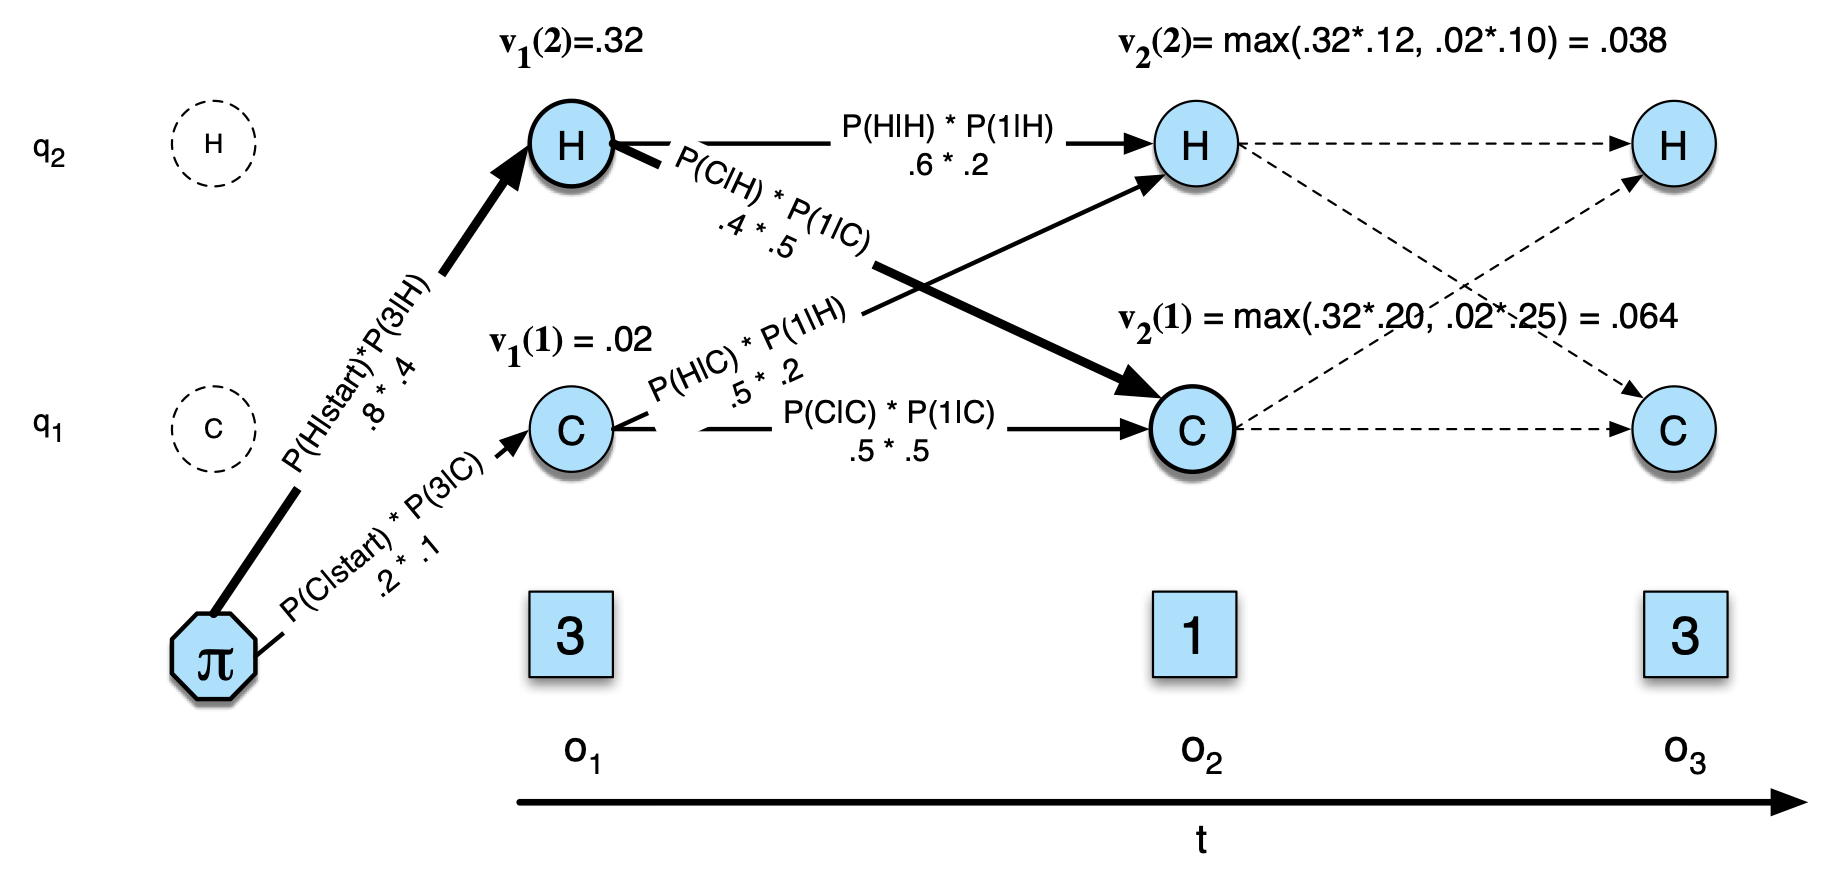
\includegraphics[width=1\textwidth]{viterbi.png}
  \caption{Viterbi trellis for computing the best path through the hidden state space for the ice-cream eating events 3-1-3. Hidden states are in circles, observations in squares. This figure is adopted from \cite{slp}}
  \label{fig:vi}
\end{figure*}


%\subsection{2.5 Gaussian Mixture Model}


\clearpage
\bigskip
\section{\textbf{3. Methods}}
\subsection{\textbf{3.1 Clustering}}


Before starting about Clustering, we should understand first what is a cluster. \footnote{This part is based on Seema Singh
 (2018) "An Introduction To Clustering". Here is the Web link \url{https://medium.datadriveninvestor.com/an-introduction-to-clustering-61f6930e3e0b}} Simply speaking,  \textbf{Cluster} is the collection of data. The data objects in one cluster are similar to one another within the same group (class or category),  and are different from the objects in the other clusters. 
The closer the objects in a cluster, the more likely they belong to the same cluster.

\begin{figure*}
 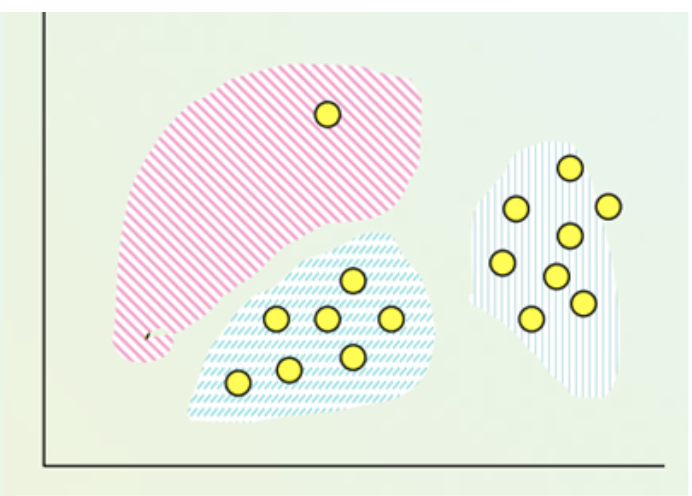
\includegraphics[width=0.6\textwidth]{clustering.png}
  \caption{clustering, adopted from \url{https://medium.datadriveninvestor.com/an-introduction-to-clustering-61f6930e3e0b}}
\end{figure*}

Based on the definition of the Cluster,  as an unsupervised learning technique in which there is predefined classes and prior information, Clustering means how the data should be grouped or labeled into separate classes. 
It could also be considered as Exploratory Data Analysis (EDA) \footnote{Exploratory Data Analysis refers to the critical process of performing initial investigations on data to discover patterns to spot anomalies to test hypothesis and to check assumptions with the help of summary statistics and graphical representations.} process which help us to discover hidden patterns of interest or structure in data. Clustering can work as a standalone tool to get the insights about the data distribution or as a preprocessing step in other algorithms.


In \cite{wang2015supervised}, they uses \textbf{Hierarchical Agglomerative Clustering} (HAC) to define segment-level features. According to \cite{chhabra2020fair}, Hierarchical Agglomerative Clustering (HAC) refers to a class of greedy unsupervised learning algorithms that seek to build a hierarchy between data points while clustering them in a bottom-up fashion. The HAC algorithm used in \cite{wang2015supervised} automatically arranges the frames in a speech segment into a tree-structured hierarchy based on the merging order of sub-segments, in which similar adjacent frames are clustered together in lower layers, while relatively dissimilar adjacent clusters are merged in higher layers. 


\subsection{\textbf{3.2 Metrics}}

There are many different metrics for evaluating clustering algorithms. 
Metrics are measures of quantitative assessment commonly used for comparing, and tracking performance or production. Metrics can be used in a variety of scenarios.  \cite{wang2015supervised}  define the pair-wise true acceptance (TA’), true rejection (TR’), false acceptance (FA’), and false rejection (FR’) for clustering tasks based on all instance pairs. Let us explain these one by one. 

The True Accept rate (TA’) is a statistic used to measure biometric performance when performing the verification task. It is the percentage of times a system (correctly) verifies a true claim of identity. While the True Reject rate (TR’) is a statistic used to measure biometric performance when performing the verification task. It refers to the percentage of times a system (correctly) rejects a false claim of identity.


False Acceptance (FA’) is the percentage of identification instances in which unauthorised persons are incorrectly accepted, and it occurs when an unauthorized subject is accepted as valid. While the False Rejection (FR') is the percentage of identification instances in which authorised persons are incorrectly rejected. As the number of false acceptances (FA') goes down, the number of false rejections (FR') will go up and vice versa.

\begin{figure*}
 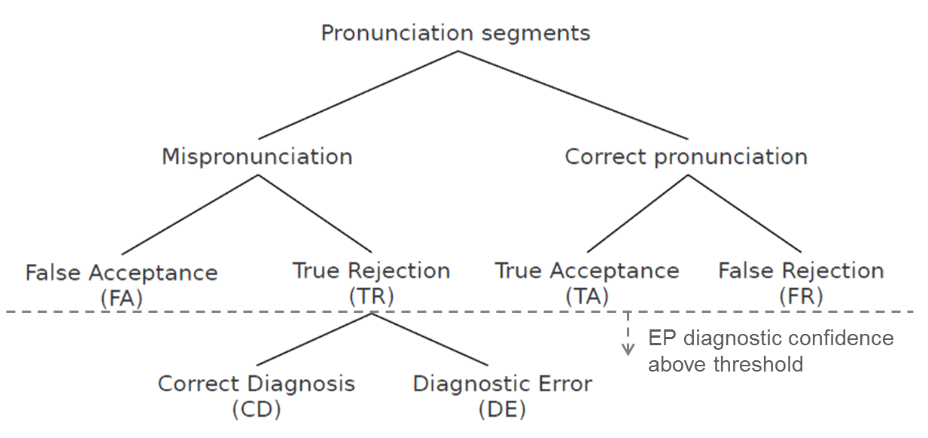
\includegraphics[width=0.6\textwidth]{metrics.png}
  \caption{Hierarchical structure of the metrics used in EP detection adopted from  \cite{wang2015supervised}}
\end{figure*}

\bigskip
\section{4. \textbf{Post-reading questions}}
In both supervised EP detection and unsupervised EP discovery, \cite{wang2015supervised} propose to utilize the universal phoneme posteriorgram (UPP), derived from a multi-layer perceptron (MLP) trained on corpora of mixed languages, but can it be applied to other datasets? And how to explain the differences of performance between the  two tasks?

%\newpage


% The Tufte-\LaTeX\ document classes define a style similar to the style Edward Tufte uses in his books and handouts.  Tufte's style is known for its extensive use of sidenotes, tight integration of graphics with text, and well-set typography.  This document aims to be at once a demonstration of the features of the Tufte-\LaTeX\ document classes and a style guide to their use.

% \section{Page Layout}\label{sec:page-layout}
% \subsection{Headings}\label{sec:headings}
% This style provides \textsc{a}- and \textsc{b}-heads (that is,
% \Verb|\section| and \Verb|\subsection|), demonstrated above.

% The Tufte-\LaTeX\ classes will emit an error if you try to use
% \linebreak\Verb|\subsubsection| and smaller headings.

% % let's start a new thought -- a new section
% \newthought{In his later books},\cite{Tufte2006} Tufte
% starts each section with a bit of vertical space, a non-indented paragraph, and sets the first few words of the sentence in \textsc{small caps}.  To accomplish this using this style, use the \Verb|\newthought| command:  
% \begin{docspec}
%   \doccmd{newthought\{In his later books\}, Tufte starts\ldots}
% \end{docspec}

% \subsection{Sidenotes}\label{sec:sidenotes}
% One of the most prominent and distinctive features of this style is the extensive use of sidenotes.  There is a wide margin to provide ample room for sidenotes and small figures.  Any \Verb|\footnote|s will automatically be converted to sidenotes.\footnote{This is a sidenote that was entered using the \texttt{\textbackslash footnote} command.}  If you'd like to place ancillary information in the margin without the sidenote mark (the superscript number), you can use the \Verb|\marginnote| command.\marginnote{This is a margin note.  Notice that there isn't a number preceding the note, and there is no number in the main text where this note was written.}

% The specification of the \Verb|\sidenote| command is:
% \begin{docspec}
%   \doccmd{sidenote[\docopt{number}][\docopt{offset}]\{\docarg{Sidenote text.}\}}
% \end{docspec}

% Both the \docopt{number} and \docopt{offset} arguments are optional.  If you
% provide a \docopt{number} argument, then that number will be used as the
% sidenote number.  It will change of the number of the current sidenote only and
% will not affect the numbering sequence of subsequent sidenotes.

% Sometimes a sidenote may run over the top of other text or graphics in the
% margin space.  If this happens, you can adjust the vertical position of the
% sidenote by providing a dimension in the \docopt{offset} argument.  Some
% examples of valid dimensions are:
% \begin{docspec}
%   \ttfamily 1.0in \qquad 2.54cm \qquad 254mm \qquad 6\Verb|\baselineskip|
% \end{docspec}
% If the dimension is positive it will push the sidenote down the page; if the
% dimension is negative, it will move the sidenote up the page.

% While both the \docopt{number} and \docopt{offset} arguments are optional, they
% must be provided in order.  To adjust the vertical position of the sidenote
% while leaving the sidenote number alone, use the following syntax:
% \begin{docspec}
%   \doccmd{sidenote[][\docopt{offset}]\{\docarg{Sidenote text.}\}}
% \end{docspec}
% The empty brackets tell the \Verb|\sidenote| command to use the default
% sidenote number.

% If you \emph{only} want to change the sidenote number, however, you may
% completely omit the \docopt{offset} argument:
% \begin{docspec}
%   \doccmd{sidenote[\docopt{number}]\{\docarg{Sidenote text.}\}}
% \end{docspec}

% The \Verb|\marginnote| command has a similar \docarg{offset} argument:
% \begin{docspec}
%   \doccmd{marginnote[\docopt{offset}]\{\docarg{Margin note text.}\}}
% \end{docspec}

% \subsection{References}
% References are placed alongside their citations as sidenotes,
% as well.  This can be accomplished using the normal \Verb|\cite|
% command.\sidenote{The first paragraph of this document includes a citation.}

% The complete list of references may also be printed automatically by using
% the \Verb|\bibliography| command.  (See the end of this document for an
% example.)  If you do not want to print a bibliography at the end of your
% document, use the \Verb|\nobibliography| command in its place.  



% \section{Figures and Tables}\label{sec:figures-and-tables}
% Images and graphics play an integral role in Tufte's work.
% In addition to the standard \docenv{figure} and \docenv{tabular} environments,
% this style provides special figure and table environments for full-width
% floats.

% Full page--width figures and tables may be placed in \docenv{figure*} or
% \docenv{table*} environments.  To place figures or tables in the margin,
% use the \docenv{marginfigure} or \docenv{margintable} environments as follows
% (see figure~\ref{fig:marginfig}):

% \begin{marginfigure}%
%   \includegraphics[width=\linewidth]{helix}
%   \caption{This is a margin figure.  The helix is defined by 
%     $x = \cos(2\pi z)$, $y = \sin(2\pi z)$, and $z = [0, 2.7]$.  The figure was
%     drawn using Asymptote (\url{http://asymptote.sf.net/}).}
%   \label{fig:marginfig}
% \end{marginfigure}
% \begin{Verbatim}
% \begin{marginfigure}
%   \includegraphics{helix}
%   \caption{This is a margin figure.}
% \end{marginfigure}
% \end{Verbatim}

% The \docenv{marginfigure} and \docenv{margintable} environments accept an optional parameter \docopt{offset} that adjusts the vertical position of the figure or table.  See the ``\nameref{sec:sidenotes}'' section above for examples.  The specifications are:
% \begin{docspec}
%   \doccmd{begin\{marginfigure\}[\docopt{offset}]}\\
%   \qquad\ldots\\
%   \doccmd{end\{marginfigure\}}\\
%   \mbox{}\\
%   \doccmd{begin\{margintable\}[\docopt{offset}]}\\
%   \qquad\ldots\\
%   \doccmd{end\{margintable\}}\\
% \end{docspec}

% Figure~\ref{fig:fullfig} is an example of the \Verb|figure*|
% environment and figure~\ref{fig:textfig} is an example of the normal
% \Verb|figure| environment.

% \begin{figure*}[h]
%   \includegraphics[width=\linewidth]{sine.pdf}%
%   \caption{This graph shows $y = \sin x$ from about $x = [-10, 10]$.
%   \emph{Notice that this figure takes up the full page width.}}%
%   \label{fig:fullfig}%
% \end{figure*}

% \begin{figure}
%   \includegraphics{hilbertcurves.pdf}
% %  \checkparity This is an \pageparity\ page.%
%   \caption{Hilbert curves of various degrees $n$.
%   \emph{Notice that this figure only takes up the main textblock width.}}
%   \label{fig:textfig}
%   %\zsavepos{pos:textfig}
%   \setfloatalignment{b}
% \end{figure}

% Table~\ref{tab:normaltab} shows table created with the \docpkg{booktabs}
% package.  Notice the lack of vertical rules---they serve only to clutter
% the table's data.

% \begin{table}[ht]
%   \centering
%   \fontfamily{ppl}\selectfont
%   \begin{tabular}{ll}
%     \toprule
%     Margin & Length \\
%     \midrule
%     Paper width & \unit[8\nicefrac{1}{2}]{inches} \\
%     Paper height & \unit[11]{inches} \\
%     Textblock width & \unit[6\nicefrac{1}{2}]{inches} \\
%     Textblock/sidenote gutter & \unit[\nicefrac{3}{8}]{inches} \\
%     Sidenote width & \unit[2]{inches} \\
%     \bottomrule
%   \end{tabular}
%   \caption{Here are the dimensions of the various margins used in the Tufte-handout class.}
%   \label{tab:normaltab}
%   %\zsavepos{pos:normaltab}
% \end{table}

% \section{Full-width text blocks}

% In addition to the new float types, there is a \docenv{fullwidth}
% environment that stretches across the main text block and the sidenotes
% area.

% \begin{Verbatim}
% \begin{fullwidth}
% Lorem ipsum dolor sit amet...
% \end{fullwidth}
% \end{Verbatim}

% \begin{fullwidth}
% \small\itshape\lipsum[1]
% \end{fullwidth}

% \section{Typography}\label{sec:typography}

% \subsection{Typefaces}\label{sec:typefaces}
% If the Palatino, \textsf{Helvetica}, and \texttt{Bera Mono} typefaces are installed, this style
% will use them automatically.  Otherwise, we'll fall back on the Computer Modern
% typefaces.

% \subsection{Letterspacing}\label{sec:letterspacing}
% This document class includes two new commands and some improvements on
% existing commands for letterspacing.

% When setting strings of \allcaps{ALL CAPS} or \smallcaps{small caps}, the
% letter\-spacing---that is, the spacing between the letters---should be
% increased slightly. The \Verb|\allcaps| command has proper letterspacing for
% strings of \allcaps{FULL CAPITAL LETTERS}, and the \Verb|\smallcaps| command
% has letterspacing for \smallcaps{small capital letters}.  These commands
% will also automatically convert the case of the text to upper- or
% lowercase, respectively.

% The \Verb|\textsc| command has also been redefined to include
% letterspacing.  The case of the \Verb|\textsc| argument is left as is,
% however.  This allows one to use both uppercase and lowercase letters:
% \textsc{The Initial Letters Of The Words In This Sentence Are Capitalized.}



\bibliography{references}
\bibliographystyle{apalike}


\end{document}